\zotelo{../thesis.bib}

\chapter{GPU architecture and CUDA}
\label{app:gpu}

% In this appendix we summarize the effective radiative drag due to resonant
% scattering in the magnetosphere of magnetars, as an extension of the physics
% model described in chapter \ref{chap:magnetar}.

\section{The GPU Architecture}
\label{sec:gpu-arch}

In the recent decade we saw the rise of GPUs or Graphics Processing Units as an
alternative way to carry out computations. GPUs are originally designed
specifically for intensive floating point calculations that are very common in
video games and 3D rendering. For these applications, typically the goal is to
compute the color of a pixel on the screen, where each pixel is relatively
independent from others. In order to compute millions of pixels every frame and
keep up with more than 60 frames per second, GPUs are designed to be massive
parallel machines. A modern GPU typically has hundreds to thousands of cores,
compared to up to less than 20 cores in a top-of-the line CPU. In terms of raw
floating point operations per second, a single modern GPU can break 5 TetraFLOPs
per second which not that many years ago was only achievable by supercomputers.
In addition, GPU comes with on-board memory which has up to 5-6 times the
bandwidth of ordinary DRAM, which further improves the computation output
especially for memory bound computation.

However, the many cores of the modern GPU come at a price, as each is less
competent than a core of an equivalent CPU. The GPU cores are organized into
symmetric multiprocessors (SMPs), and all the cores in an SMP share one control
unit while each core has only an ALU (Arithmetic Logic Unit) which is used to
perform arithmetic and logic operations (figure \ref{fig:gpu-vs-cpu}). This
means that the same statement is carried out not by only one core but by a group
of cores, on a chunk of data at the same time. At the time of this writing, the
popular Nvidia K40 processor is the most common one found in local and national
clusters. It has 15 SMPs each with 192 CUDA cores, giving a total of 2880 cores.

\begin{figure}[h]
  \centering
  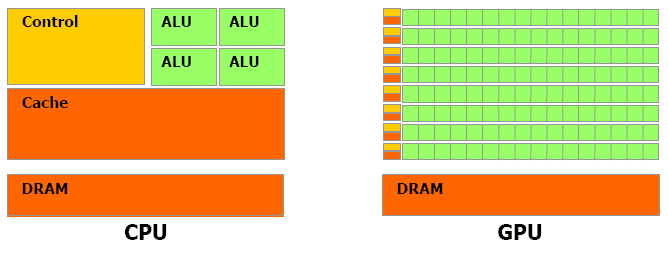
\includegraphics[width=0.7\textwidth]{pics/appendix/gputech_f2.png}
  \caption{Difference in GPU and CPU internal structure.}
  \label{fig:gpu-vs-cpu}
\end{figure}

This particular architecture is perfect for operations that naturally calls for
parallelism, but poses a serious programming challenge for general tasks. For
example, when an algorithm requires iterations where each step depends on the
previous one (e.g. numerical integration of an ODE), there is no way to do it in
parallel, and the GPU structure falls back to executing everything in series,
which is very slow due to the inherently lower clock speed. Another problem lies
deeper in the architecture itself. The many cores in an SMP are organized into
``warps'' of typically 32 cores each. An instruction is passed to a warp and
executed by all 32 cores simultaneously regardless of the content of the
instruction or any conditional statements. If an \verb!if! statement is part of
the instruction and segregates the warp into two branches, then the two branches
will both be executed by all threads, with inappropriate results discarded. The
worst case is when all 32 instances belong to different conditional branches,
the same instructions will be executed 32 times, effectively erasing any
parallelization.

The GPU version of Aperture is developed using the CUDA parallel computing
platform, created by Nvidia Corporation, and designed to be executed on Nvidia
GPUs. The CUDA platform is a software layer that gives direct access to the
GPU's virtual instruction set and parallel computational elements, for the
execution of compute kernels. CUDA is designed to work with programming
languages such as C, C++, and Fortran. Since Aperture was developed in C++, it
is natural to blend CUDA into the code base. In the remaining part of this
appendix, we will describe the execution model of CUDA and outline how I
designed Aperture to take advantage of this model.

\section{The CUDA execution model}
\label{sec:cuda-model}

As mentioned in section \ref{sec:gpu-arch}, GPU relies on massive
parallelization for its speed advantage over ordinary CPUs. This is explicitly
built into the execution model of CUDA. Functions allowed to run on the GPU are
called compute kernels, and are annotated with the keyword \verb!__global__! in
front of the function definition. When a compute kernel is launched, a set of
additional parameters is given specifying the number of threads that will
execute the kernel in parallel. It is very typical to launch hundreds of
thousands of threads at the same time.

Threads in CUDA are organized into thread blocks. Each thread block can have at
most 1024 threads. Multiple blocks can be launched at the same time, and there
is no upper limit on the number of blocks launched. At execution time, thread
blocks are assigned to SMPs. On K40 up to 16 blocks can be sent to an SMP at a
time, and each block is executed in warps of 32 threads. For example, if a
compute kernel is launched with 128 blocks of 512 threads each, in reality up to
64 randomly chosen warps from 16 blocks can be executed at the same time for
each SMP, and it is all up to the scheduler in the SMP to decide at runtime.

Apart from the warp execution model, each thread block also has a small pool
called ``shared memory'' that is accessible by all threads inside the block.
This piece of shared memory is similar to the L1 cache in ordinary
CPUs\footnote{In fact, the user can choose how the 64KB is split between L1
  cache and the shared memory.}, which has very low latency compared to the main
memory. In addition, threads in a given block can write to the shared memory
{\it atomically}, avoiding race condition. The same operation is much more
costly and difficult to do on the main memory. In K40 each block can have up to
64KB of shared memory. If all threads in a block access a common part of the
main memory repeatedly, loading that part of main memory into shared memory
first can accelerate the memory access speed by a factor of more than a hundred.

In general, memory speed is an important aspect of the GPU program design. The
different levels of memory accessible to a program forms a hierarchy in terms of
speed and latency. The system RAM is the slowest, since every access from the
GPU need to go through the PCIe bus, which has a latency of $\sim 1000$ cycles
and a bandwidth of only a fraction of the system RAM bandwidth. The on board GPU
memory\footnote{The on board GPU memory is called ``global memory'' in CUDA.}
does not suffer from this issue, and due to design its bandwidth is much higher
than the system RAM, however it still suffers from very high latency: an access
to the GPU main memory requires $\sim 200$ clock cycles. A faster but very
limited memory space is the L1 cache/shared memory as mentioned above. An access
to the shared memory only has latency of a few clock cycles, and multiple
threads reading the same address can be done in a single operation.
Figure % TODO: figure
shows the GPU memory hierarchy and the perspective memory bandwidth/latency.

\begin{figure}[h]
  \centering

  \caption[Memory hierarchy of Nvidia GPUs.]{Memory hierarchy of Nvidia GPUs.}
  \label{fig:gpu-memory}
\end{figure}

Therefore the optimal strategy is to either keep all the computation data on GPU
main memory, or to overlap memory copy with computation as much as possible.
When processing data on GPU main memory, try to manipulate a local block of data
at a time by loading them to the shared memory of a thread block, do the
calculation in parallel compute kernels, and then save them back to the GPU main
memory.

\section{Parallelization and optimization in Aperture}
\label{sec:optimization}

PIC codes are naturally very suited for GPUs due to the algorithm being readily
parallelizable. A PIC code typically deals with millions to billions of
particles, each relatively independent of each other especially for
collisionless plasma. On a grid scale, the Maxwell solver is also typically
parallel, each cell only requires the information of a few adjacent cells and
updates independently. Moreover, GPU excels at floating point operations which
is the main kind of arithmetic operations used in a PIC code. The only
potential problem for parallelization lies in current deposition, where by
definition multiple particles need to be processed and then write the result to
the same cell, which can only be done serially.

\subsubsection{Particle pusher}
\label{sec:gpu-pusher}

Most of the particle pusher algorithm is completely parallelizable. Given the
values of $E$ and $B$ fields at the particle location, every particle can be
processed independently to update their momenta and positions. This lend itself
well to the parallel structure of GPUs. The only nontrivial optimization is to
interpolate the field values to particle position, which involves frequent random
access to the field array which is not a strength of the GPU architecture.

The way we optimize this part of the code is to subdivide the whole
computational domain in ``tiles'', such that the 6 field components of each tile
can fit into the shared memory of a thread block. In 2D simulations we found
that $8\times 8$ tiles works very nicely. In the compute kernel, a thread block
is assigned to every tile in the domain, and the threads first load the $E$ and
$B$ field values from global memory into the shared memory of the block. Then
the threads in the block work through the particles inside the tile in parallel,
interpolating the field values to the local particle position using the values
in the shared memory, then update the particle momentum using Vay pusher
(section \ref{sec:ptc-pusher}).

% TODO: A graph or pseudo code to demonstrate the process

A small sacrifice for this algorithm is that we need to have the particles
sorted by tile all the time. Therefore at each time step we sort them
immediately after particle move and production of new pairs, since both
operations mess up the particle order: movement between tile boundary, and
because all new particles are added to the end of the particle array. However we
found this to be the best way since current deposition also benefits from having
a sorted particle array (see \ref{sec:gpu-deposit}).

\subsubsection{Current deposition}
\label{sec:gpu-deposit}

Current deposition poses a main problem for a massively parallelized
architecture like the GPU, since by definition many threads (particles) need to
write the same memory location (current values on the grid), which can not be
done in parallel.

\subsubsection{Pair creation}
\label{sec:gpu-pair}

Pair creation poses a similar problem as current deposition. Since new particles
are appended to the end of the main particle array, every photon that is to
convert to a pair will need to access the end of the array and race condition
may occur unless the process is serialized.



% Local Variables:
% TeX-master: "../thesis"
% zotero-collection: #("16" 0 2 (name "Thesis"))
% End:
